\section{Proposed SCL Framework}\label{sec:method}

\scl{} is a lightweight, rule-based layer operating between a frozen detector and tracker (the
host) without modifying their underlying algorithms. Fig.~\ref{fig:arch} illustrates the five
processing steps of \scl{} for frame $t$. First, Otsu-based logit partitioning (Step~1) divides
recent detection scores into background, uncertain, and confident groups. Next, detection stream
classification (Step~2) determines whether the score distribution is clean or noisy based on
historical confidence statistics. Mode-adaptive candidate selection (Step~3) then retains,
removes, or remaps detection scores and adjusts the tracker's confidence thresholds according to
the operating mode. Track-guided weak detection recovery (Step~4) allows eligible low-confidence
detections to support track continuity. Finally, camera motion-adaptive matching tolerance
(Step~5) adjusts the association criterion according to estimated camera motion. The host
contract provides the tracker's published parameters, while the tracker performs its original
association and track-management operations unchanged.

Table~\ref{tab:symbols} lists every symbol in plain words, with its value in the clean stream of
Fig.~\ref{fig:groups}a, which the subsections below follow from input to output.

\begin{table*}[!tb]
\caption{The symbols of Sect.~\ref{sec:method} in plain words. Example: the value in the clean
stream of Fig.~\ref{fig:groups}a (MOT17-02, frame 101, ByteTrack in its official setting), as
recorded by the frozen \scl{}; e.g.: a worked example from the text.}
\label{tab:symbols}
\centering\footnotesize
\setlength{\tabcolsep}{3pt}
\begin{tabular}{@{}l>{\raggedright\arraybackslash}p{97mm}>{\raggedright\arraybackslash}p{40mm}@{}}
\toprule
Symbol & Meaning & Example\\
\midrule
$s_i$, $z_i$ & detector score of candidate $i$, between 0 and 1, and its logit, Eq.~\eqref{eq:logit} & e.g.\ 0.9 and $\log 9=2.2$\\
$W$, $Z_t^W$ & number of past frames whose logits are pooled; the logits of frames $t-W$ to $t-1$ & 10; 916 logits\\
$t_1$, $t_2$ & first split (background lies below it); second split (confident lies above it) & $-0.78$ (0.32); 0.95 (0.72)\\
$\rho_t$ & share of confident candidates in the foreground, Eq.~\eqref{eq:rho} & $175/263=0.67$\\
median $\rho$ & median of $\rho$ over the stream so far; clean if $\ge0.5$ & 0.63: clean\\
$a$, $b$, $\ell$ & the tracker's published scores to match a track and to start one, and the lowest score it uses & 0.6, 0.7, 0.1\\
$m_0$ & the tracker's matching tolerance: 1 minus the smallest IoU that matches & 0.8 (IoU $\ge0.2$)\\
$a_t$, $b_t$, $m_t$ & the thresholds and tolerance \scl{} passes for frame $t$, Eqs.~\eqref{eq:clean} and~\eqref{eq:motion} & 0.6, 0.7 (kept); 0.8\\
$u_i$, $\tilde{s}_i$ & rank of $s_i$ among stored scores; the new score of the noisy mode, Eq.~\eqref{eq:remap} & e.g.\ $u_i=0.8\to\tilde{s}_i=0.9$\\
$\mathcal{T}_{t-1}$, $K_t$ & the tracks of the previous frame; the candidates passed to the tracker & --\\
$g_t$, $r_t$ & camera shift between two frames; its ratio to the usual shift & e.g.\ $r_t=2$\\
\bottomrule
\end{tabular}
\end{table*}


\subsection{Inputs and outputs of SCL}\label{sec:problem}
In each frame $t$, the detector gives candidates $D_t=\{(\mathbf{x}_i,s_i,c_i)\}$, each with a box
$\mathbf{x}_i$, a score $s_i\in(0,1)$, and a class $c_i$. The layer works on the logit
\begin{equation}
z_i=\log\frac{s_i}{1-s_i},
\label{eq:logit}
\end{equation}
which keeps the order of the scores (0.5 gives $z_i=0$, 0.9 gives $\log9=2.2$, and 0.1 gives $-2.2$)
and spreads out the regions near 0 and 1, where detector scores crowd; the logistic function
$\sigma(z)=1/(1+e^{-z})$ maps a logit back to a score. The host gives its contract $h=(a,b,\ell,m_0)$:
the score $a$ needed to match a track, the score $b$ needed to start one, the lowest score $\ell$ it
uses, and its matching tolerance $m_0$, one minus the smallest intersection over union (IoU) that
counts as a match. A single-stage tracker has $\ell=\min(a,b)$, a two-stage tracker $\ell<\min(a,b)$.
For ByteTrack in its official setting, $a=0.6$, $b=0.7$, $\ell=0.1$, and $m_0=0.8$
(Table~\ref{tab:contracts}). In every frame the layer returns
\begin{equation}
\left(K_t,\tilde{s},a_t,b_t,m_t\right)=
\mathcal{L}\left(Z_{<t},D_t,\mathcal{T}_{t-1},g_t;\,h\right):
\label{eq:layer}
\end{equation}
the candidates $K_t$, their scores, and the thresholds and tolerance for the tracker, from the logits
$Z_{<t}$ of earlier frames, the tracks $\mathcal{T}_{t-1}$, and the camera motion $g_t$ between frames
$I_{t-1}$ and $I_t$; no future frame is used.

\begin{table*}[!t]
\caption{Host contracts: the four published settings $(a,b,\ell,m_0)$ of each tracker that \scl{}
reads (Sect.~\ref{sec:problem}), and where each value comes from; $\theta$: the published IoU
threshold, $m_0=1-\theta$.}
\label{tab:contracts}
\centering\footnotesize
\setlength{\tabcolsep}{4pt}
\begin{tabular}{@{}llcccc>{\raggedright\arraybackslash}p{84mm}@{}}
\toprule
Tracker (setting) & Type & $a$ & $b$ & $\ell$ & $m_0$ & Published settings behind the values\\
\midrule
ByteTrack (official) & two-stage & 0.6 & 0.7 & 0.1 & 0.8 & track\_thresh 0.6; new tracks $+$0.1; second step from 0.1; match\_thresh 0.8\\
ByteTrack (library) & two-stage & 0.25 & 0.25 & 0.1 & 0.8 & Ultralytics bytetrack.yaml: high 0.25, new 0.25, low 0.1, match 0.8\\
BoT-SORT (library) & two-stage & 0.25 & 0.25 & 0.1 & 0.8 & Ultralytics botsort.yaml: the same four values\\
SparseTrack & two-stage & 0.6 & 0.7 & 0.1 & 0.85 & track\_thresh 0.6; new tracks $+$0.1; second step from 0.1; match\_thresh 0.85\\
BoostTrack & two-stage & 0.6 & 0.6 & 0.1 & 0.7 & det\_thresh 0.6; every detection from 0.1 can be boosted; $\theta=0.3$\\
Hybrid-SORT & two-stage & 0.6 & 0.6 & 0.1 & 0.75 & det\_thresh 0.6; low-score step from 0.1; $\theta=0.25$\\
OC-SORT & single-stage & 0.6 & 0.6 & 0.6 & 0.7 & det\_thresh 0.6, no low-score step; $\theta=0.3$\\
PD-SORT & single-stage & 0.6 & 0.6 & 0.6 & 0.7 & det\_thresh 0.6, no low-score step; $\theta=0.3$\\
\bottomrule
\end{tabular}
\end{table*}


\subsection{Otsu-Based Logit Partitioning and Confidence Estimation}\label{sec:calib}
\emph{Step 1 in Fig.~\ref{fig:arch}. Input:} the logits $Z_t^W$ of the candidates of the last $W=10$
frames. \emph{Output:} the splits $t_1$, $t_2$ and the confident share $\rho_t$.

The logits are split twice with Otsu's method \cite{goh2018otsu}, which picks from the data alone the
threshold that best separates two groups: $t_1$ separates background (low logits) from foreground,
and $t_2$, found on the foreground only, divides it into uncertain and confident candidates. The
share of confident candidates in the foreground,
\begin{equation}
\rho_t=\frac{\left|\{z\in Z_t^W: z\ge t_2\}\right|}{\left|\{z\in Z_t^W: z\ge t_1\}\right|},
\label{eq:rho}
\end{equation}
describes the shape of the score distribution. In the clean stream of
Fig.~\ref{fig:groups}a, the window holds 916 candidates: 653 below $t_1=-0.78$ (score 0.32), 88
between the splits, and 175 above $t_2=0.95$ (score 0.72), so $\rho_t=175/(88+175)=0.67$; in the
noisy stream of Fig.~\ref{fig:groups}b, 1,037 are background, 99 uncertain, and 83 confident, so
$\rho_t=83/(99+83)=0.46$. As clutter usually gives more candidates than objects do, a window with
fewer candidates below $t_1$ than above it counts as clean, $\rho_t=1$ (background check), which does
not apply in Fig.~\ref{fig:groups}.

\begin{figure}[t]
\centering
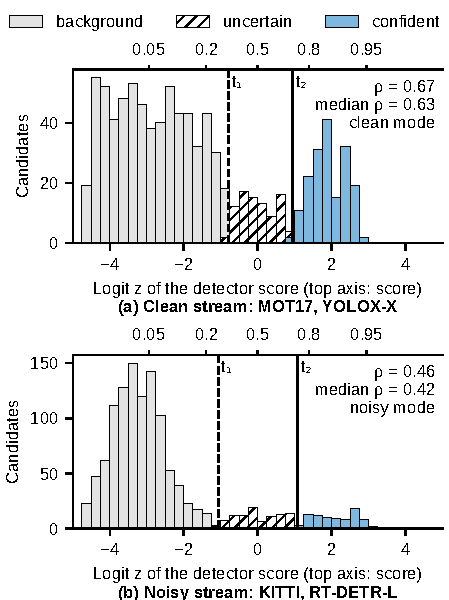
\includegraphics{Fig2.pdf}
\caption{What \scl{} sees before its decision for frame 101: the logits of the candidates of the last
10 frames (top axis: the same position as a score). Dashed line: $t_1$; solid line: $t_2$; light gray:
background; hatched: uncertain; blue: confident. (a) MOT17 sequence MOT17-02, YOLOX-X, ByteTrack
(official): median $\rho=0.63\ge0.5$, clean. (b) KITTI sequence 0001, RT-DETR-L, ByteTrack (library):
median $\rho=0.42<0.5$, noisy. Values recorded by the frozen \scl{}}
\label{fig:groups}
\end{figure}

\subsection{Median-Based Detection Stream Classification}\label{sec:regimes}
\emph{Step 2 in Fig.~\ref{fig:arch}. Input:} the values $\rho$ of all frames so far. \emph{Output:}
the mode of frame $t$.

The mode describes the distribution of the scores, not whether a single detection is correct: the
stream is clean at frame $t$ if the median of all $\rho$ values so far is at least one half, a
majority rule, and noisy otherwise; before the first valid split it is cold. In
Fig.~\ref{fig:groups}a, frames 2 to 101 give a median of 0.63, so frame 101 is clean; in
Fig.~\ref{fig:groups}b the median is 0.42, so it is noisy. The whole-stream median keeps the mode
stable against a few frames of blur or occlusion, while the groups, and in the clean mode the
thresholds of Step~3, follow a new score scale within $W$ frames.

\subsection{Mode-Adaptive Detection Candidate Selection and Threshold Adjustment}\label{sec:choice}
\emph{Step 3 in Fig.~\ref{fig:arch}. Input:} $D_t$, the mode, $t_1$, $t_2$, the thresholds $a$, $b$,
and the tracks $\mathcal{T}_{t-1}$. \emph{Output:} the kept boxes, their scores, and the thresholds
$a_t$, $b_t$.

\emph{Cold and clean modes.} The tracker keeps its own scores, and only cross-class duplicates are
removed. In the clean mode, a threshold that would reject the confident group is lowered to the
score $\sigma(t_2)$ at which that group begins:
\begin{equation}
a_t=\min\!\left(a,\sigma(t_2)\right),\qquad b_t=\min\!\left(b,\sigma(t_2)\right).
\label{eq:clean}
\end{equation}
In Fig.~\ref{fig:groups}a, $\sigma(t_2)=0.72$ is above both $a=0.6$ and $b=0.7$, so the published
thresholds are kept and the output equals that of the host alone (Sect.~\ref{sec:results}). When the
scores are halved, no score is above 0.5 and ByteTrack in its official setting never starts a track;
$\sigma(t_2)$ falls with the scores below 0.5, Eq.~\eqref{eq:clean} lowers both thresholds to it, and
the confident candidates reach the tracker again.

\emph{Noisy mode.} Background candidates ($z<t_1$) are dropped. Each remaining score is replaced by
its mid-rank $u_i\in(0,1)$ among the scores of a remap memory, which stores the scores kept in the
first frame and in every 10th frame, the last 20 of them (equal scores count half):
\begin{equation}
\tilde{s}_i=
\begin{cases}
0.5+0.5\,u_i, & z_i\ge t_2,\\
0.1+0.4\,u_i, & t_1\le z_i<t_2,
\end{cases}
\label{eq:remap}
\end{equation}
and both thresholds are set to $a_t=b_t=0.5$. A confident candidate with $u_i=0.8$ gets
$0.5+0.5\cdot0.8=0.9$ and may start and continue tracks; an uncertain one with $u_i=0.3$ gets
$0.1+0.4\cdot0.3=0.22$ and may only continue tracks through a tracker's low-score step. A weaker
candidate that overlaps a stronger one with IoU above one half is removed, unless a different track of
the previous frame claims it, which keeps people who stand close together in a crowd.

\emph{Score remapping is not probability calibration.} Calibration learns from labelled data the
probability that a detection is correct \cite{kuppers2020detcalib}. The remap needs no labels: it
keeps the order of the scores within each group and places the groups in fixed ranges, so that the
tracker's own thresholds read the layer's decision (above 0.5: ``may start a track''; 0.1 to 0.5:
``may only continue one''), and it is unchanged by any order-preserving change of the scores.

\subsection{Track-Guided Weak Detection Recovery}\label{sec:rescue}
\emph{Step 4 in Fig.~\ref{fig:arch}. Input:} the output of Step~3, the tracks $\mathcal{T}_{t-1}$,
and $\ell$. \emph{Output:} $K_t$, their scores, and $a_t$, $b_t$ for the tracker.

A track can be lost when its object gets low scores for a few frames, above all in a single-stage
tracker, which has no low-score step. The rescue passes such a candidate, with its score raised just
above the lowest threshold of the frame ($\ell$ for a two-stage tracker, the lower of $a_t$ and $b_t$
for a single-stage one), when it is in the foreground (or, for a single-stage tracker, when there is
no background group), overlaps a track of the previous frame with IoU of at least one half, no other
usable candidate covers that track, and the tracker could not see it otherwise. For ByteTrack in its
official setting, a rescued candidate gets $0.101$ and enters its low-score step; for OC-SORT in a
noisy frame it gets $0.501$. The tracker itself still decides, with its own matching, whether and to
which track the box is assigned.

\subsection{Camera Motion-Adaptive Matching Tolerance}\label{sec:motion}
\emph{Step 5 in Fig.~\ref{fig:arch}. Input:} the frames $I_{t-1}$, $I_t$ and the tolerance $m_0$.
\emph{Output:} the tolerance $m_t$ of frame $t$.

In noisy frames, the matching tolerance grows with camera motion, which moves boxes far from their
tracks; otherwise $m_t=m_0$. The motion $g_t$ is the shift between consecutive grayscale
frames at quarter resolution, found by phase correlation \cite{tong2019fourier}, and $r_t$ is its
ratio to its median over the last 100 frames ($r_t=1$ during a warm-up of 5 frames or if this median
is zero):
\begin{equation}
m_t=\min\!\left(0.95,\;1-\frac{1-m_0}{\max(1,r_t)}\right).
\label{eq:motion}
\end{equation}
With $m_0=0.8$, a match needs an IoU of at least 0.2; if the camera moves twice as much as usual
($r_t=2$), then $m_t=\min(0.95,\,1-0.2/2)=0.9$, and an IoU of 0.1 is enough. The cap 0.95 keeps a
smallest overlap of 0.05.

\subsection{SCL Integration with Existing Trackers}\label{sec:contract}
Each contract value in Table~\ref{tab:contracts} comes from the tracker's published configuration;
none is fitted. For each tracker family, a small adapter writes the layer's outputs into the
tracker's existing parameters and calls its own update, so the authors' matching, motion model,
track management, and post-processing run unchanged.


\begin{table}[!tb]
\caption{The fixed values of \scl{}, their settings, and their sources; the same values are used for every tracker, detector, and dataset.}
\label{tab:constants}
\centering\footnotesize
\setlength{\tabcolsep}{3pt}
\begin{tabular}{@{}>{\raggedright\arraybackslash}p{23mm}>{\raggedright\arraybackslash}p{29.5mm}>{\raggedright\arraybackslash}p{19mm}@{}}
\toprule
Value & Setting & Source\\
\midrule
Window $W$ & 10 frames & design choice\\
Mode rule & clean if median $\rho\ge0.5$ & majority rule\\
Background check & $\rho=1$ if fewer below $t_1$ & no background\\
Noisy score ranges & $[0.5,1)$, $[0.1,0.5)$ & common values\\
Noisy $a_t$, $b_t$ & 0.5 & common value\\
Remap memory & 20 frames, every 10th & design choice\\
Duplicate, rescue IoU & 0.5 & MOT evaluation\\
Rescued score & lowest threshold $+\,0.001$ & just above it\\
Motion cue & phase correlation, $\tfrac{1}{4}$ size & standard \cite{tong2019fourier}\\
Motion history & 100 frames, warm-up 5 & design choice\\
Tolerance cap & 0.95 & overlap $\ge0.05$\\
\bottomrule
\end{tabular}
\end{table}

\subsection{Fixed SCL Parameters}\label{sec:constants}
Table~\ref{tab:constants} lists all values of \scl{}. They were fixed before the external
evaluation, and none was chosen by searching over a range of values: they are standard values (the
IoU of 0.5 of MOT evaluation and the common thresholds 0.5 and 0.1), definitions, or design choices
kept fixed in all development stages. Algorithm~\ref{alg:layer} gives Steps 1--5 for one frame.

\begin{algorithm}[t]
\caption{\scl{} for frame $t$; the comments name the steps of Fig.~\ref{fig:arch}. The window
holds the logits of frames $t-W$ to $t-1$, so the decision for frame $t$ uses no future frame.}\label{alg:layer}
\begin{algorithmic}[1]
\Require candidates $D_t$, tracks $\mathcal{T}_{t-1}$, motion cue $g_t$, contract $(a,b,\ell,m_0)$, constants of Table~\ref{tab:constants}
\Ensure candidates $K_t$, scores $\tilde{s}$, thresholds $a_t,b_t$, tolerance $m_t$
\State $z_i\gets$ logit of $s_i$ for all $i$ \Comment{Eq.~\eqref{eq:logit}}
\If{no valid split exists} \Comment{e.g., first frame}
  \State mode $\gets$ cold; $(a_t,b_t)\gets(a,b)$
\Else
  \State $(t_1,t_2)\gets$ nested Otsu on the window \Comment{Step 1}
  \State $\rho_t\gets$ Eq.~\eqref{eq:rho} with the background check
  \State mode $\gets$ clean if $\mathrm{median}(\rho)\ge0.5$, else noisy \Comment{Step 2}
\EndIf
\If{mode is cold or clean} \Comment{Step 3}
  \State remove cross-class duplicates; keep raw scores
  \State if clean, set $(a_t,b_t)$ by Eq.~\eqref{eq:clean}
\Else \Comment{noisy mode}
  \State remove duplicates with track context
  \State drop $z<t_1$; remap by Eq.~\eqref{eq:remap}; $a_t,b_t\gets0.5$
\EndIf
\State rescue continuations (not cold) \Comment{Step 4}
\State $m_t\gets$ Eq.~\eqref{eq:motion} if noisy, else $m_0$ \Comment{Step 5}
\State pass $K_t$, $\tilde{s}$, $a_t$, $b_t$, $m_t$ to the tracker
\State update the window (logits left after duplicate removal), the motion history ($g_t$), and the stored tracks after the tracker update
\end{algorithmic}
\end{algorithm}

